%!TEX root = ../main.tex
\documentclass[../main.tex]{subfiles}
\begin{document}
  \chapter{Characteristic Based Population Models}\label{chapter:derivation}

  In this chapter we consider the models in \cite{mckendrick1926} and \cite{foerster1959} who describe a system indexed by age. We then consider of the advances in \cite{silvert1978} who describe new equations indexed by weight and the derive the standard McKendrick-von Foerster Equation for weight indexed systems.

  This work serves as the basis for \cite{datta2010}, who constructs a stochastic model for the dynamics of population, which they call the deterministic jump-growth equation. We consider the relevance of this equation in relation to the McKendrick-von Foerster Equation drawing further on the work of \cite{datta2010}.

  \section{Age Indexed Models}
  \cite{mckendrick1926} first posed the idea of modeling biological processed for medicinal science by a single characteristic. In a process of individuals meet they transfer information within the system, and if one considers these as individuals as particles in a system moving according to a dimension indexed by this single characteristic then their movement becomes a study in kinetics.

  \cite{foerster1959} extended the principle equations derived in \cite{mckendrick1926} with extensions. \cite{trucco1965} gives a full rigorous discussion of the advancements made in \cite{foerster1959}. It's discussion involve considering the steady state solutions of what he calls ``The Von Foerster Equation'', which we discuss further in Section~\ref{sec:mvf:steadystate}.

  \subsection{The Von Foerster Equation}
  \begin{equation}\label{eq:mvf:vfeq}
    \frac{\partial n}{\partial t} + \frac{\partial n}{\partial a} = - m(a)n
  \end{equation}

  Following the work of \cite{trucco1965} we now describe Von Foerster's reasoning to determine Equation~\ref{eq:mvf:vfeq}. Suppose that $n(t, a)$ represents the density of individuals at time $t$ in the age category $(a, a + \Delta a)$. Then we have that
  \begin{eqnarray}\label{eq:mvf:derivword}
    \frac{\partial}{\partial t} \left( n(a, t) \Delta a \right)
    &=& + \mbox{ rate of entry of } a \nonumber \\
    &=& - \mbox{ rate of departure at } (a + \Delta a) \nonumber \\
    &=& - \mbox{ deaths in } (a, a + \Delta a).
  \end{eqnarray}

  We can express which in mathematical terms for some \emph{flux}, $J(t, a)$, which describes that rate of movement of individuals in $(a, a + \Delta a)$ as
  \begin{equation}\label{eq:mvf:flux}
    \frac{\partial n}{\partial t} = \frac{J(t, a) - J(t, a + \Delta a)}{\Delta a} - m(a) n(a, t).
  \end{equation}

  for some per capita mortality rate $m$. When dealing with the flux $J$ we consider that this represents the movement of individuals in age. As individuals become older the flux can be assumed the be proportional to the density of individuals with some velocity $v(t, a)$. If the aging corresponds to the parsing of time then we have that
  $$ v = \frac{\partial a}{\partial t} = 1$$

  and so $J(t, a) = n(t, a)$. Substituting this in it is clear that, in the limit as as $\Delta a \to 0$, Equation~\ref{eq:mvf:flux} becomes the von Foerster Equation (\ref{eq:mvf:vfeq}).

  \section{Weight Indexed Models}
  \subsection{McKendrick-von Foerster Equation}
  \cite{silvert1978} introduced a more general construction of the McKendrick-von Foerster Equation, notwithstanding a change from age indexed population to sized based population, in a model which allowed growth and mortality to be functions of body mass. Their changes are widely used in mathematical biology and a full derivation can be found in \cite{silvert1978}, however a simple argument is that the \emph{flux} described in Equation~\ref{eq:mvf:flux} is changed for a flux that depends on the growth of individuals
  $$J(t, w) = g(t, w)n(t, w)$$

  and $m(a)$ becomes a mortality function in weight and age $\mu(w)$. Thus the McKendrick-von Foerster Equation reads
  \begin{equation}\label{eq:mvf:mvf}
    \frac{\partial n}{\partial t} + \frac{\partial}{\partial w} \left(g \cdot n \right) = - \mu \cdot n.
  \end{equation}

  \subsection{Jump Growth Equation}
  While the mathematical framework presented in \cite{silvert1978}, \cite{datta2010} presents a different method of describing weight indexed population under a the assumption that predation is a Markov process. The predation event extends the ideas of \cite{silvert1980} where predation is modeled the coupled death at one size to the growth of another. This is illustrated in Figure~\ref{fig:mvf:predation} where we see there are three types of predation to yield news individuals weight $w_c$.

  \begin{figure}
    \centering
    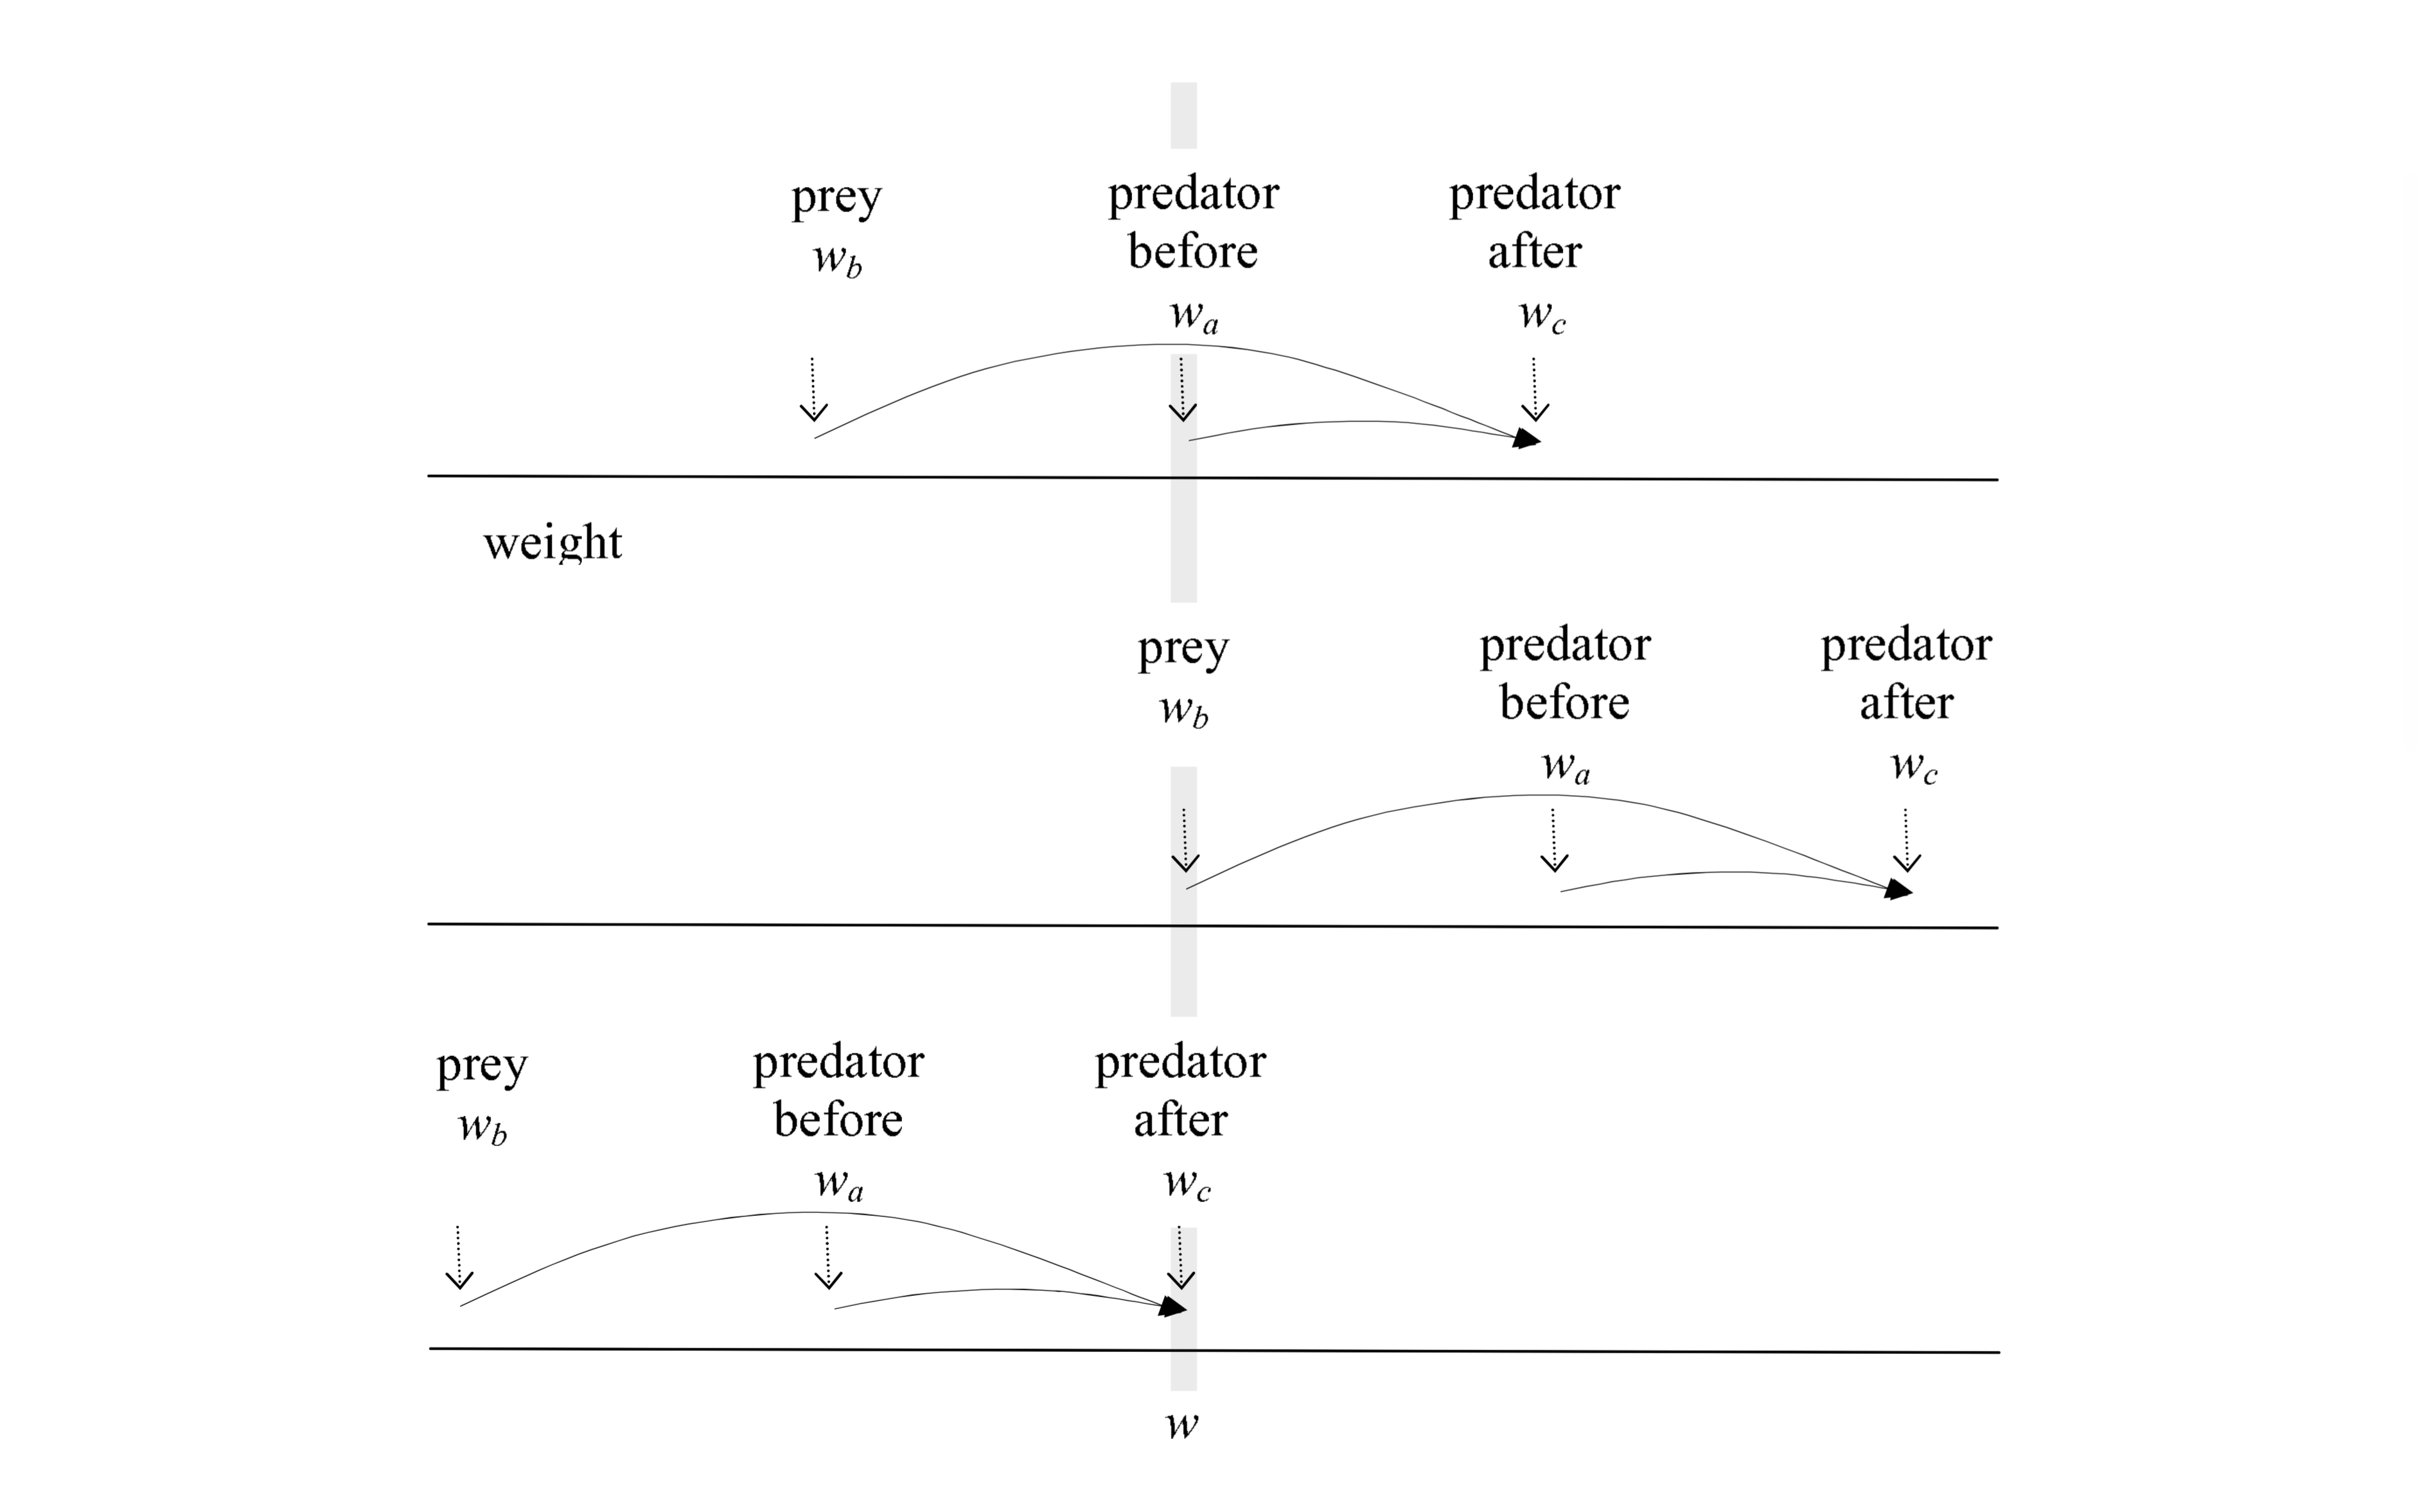
\includegraphics[width=0.75\textwidth]{img/stochastic_predation.png}
    \caption{Figure 1 from \cite{datta2010}. The death of an individual with weight $w_b$ is attributed to the growth of another individual weight $w_a$, who consequently dies to yield a new individual with weight $w_c = w_a + K w_b$ for some predation efficiency $K$ that could be a function of weight. \label{fig:mvf:predation}}
  \end{figure}

  \begin{align}\label{eq:mvf:jump}
    \frac{\partial \phi(w)}{\partial t}
    = \int ( &- k(w, w') \phi(w)\phi(w') \nonumber \\
    & - k(w, w')\phi(w')\phi(w) \nonumber \\
    & + k(w - Kw', w')\phi(w - Kw')\phi(w')) \: \mathrm{d}w'.
  \end{align}

  The research in \cite{datta2010} yields the ``Deterministic Jump-Growth Equation'', an analytic partial differential equation derived from the macroscopic stochastic models. Equation~\ref{eq:mvf:jump} represents this model, where $K$ is the predation efficiency and $k(w, w')$ is the feeding rate for individuals weight $w$ feeding on individuals weight $w'$.

  \subsection{Relation of Jump Growth Equation and McKendrick-von Foerster Equation}\label{sec:mvf:relation}
  \cite{law2009} shows that under the assumption of stochastic predation that Equation~\ref{eq:mvf:mvf} is a suitable model for population dynamics under the assumption that the growth rate of an individual with weight $w$ from feeding on smaller organizations can be expressed as
  \begin{equation}
    G(w) = \int K w' k(w, w') \phi(w') \: \mathrm{d}w',
  \end{equation}

  and similarly the per capita mortality rate at weight $w$ is modelled as
  \begin{equation}
    \mu(w) = \int k(w', w) \phi(w') \: \mathrm{d}w'.
  \end{equation}

  \cite{datta2010}, Chapter 2.5, shows that this model can be shown as an approximation to Equation~\ref{eq:mvf:jump}. By expanding the Taylor series of the last term of Equation~\ref{eq:mvf:jump} we see that

  \begin{eqnarray}\label{eq:mvf:diffusion}
    \frac{\partial \phi(w)}{\partial t}
    &=& \int k(w', w) \phi(w)\phi(w') \: \mathrm{d}w' \nonumber \\
    && - \frac{\partial}{\partial w} \int K w' k(w, w')\phi(w')\phi(w) \: \mathrm{d}w' \nonumber \\
    && + \frac{1}{2} \frac{\partial}{\partial w} \int (K w')^2 k(w, w')\phi(w')\phi(w)  \: \mathrm{d}w' \nonumber \\
    && + R,
  \end{eqnarray}

  for a remainder term $R$. Clearly the first two terms correspond the McKendrick-von Foerster Equation. Therefore in our method for constructing a numerical scheme for the Jump Growth Equation we will focus on Equation~\ref{eq:mvf:diffusion}, which we call the Growth-Diffusion Equation, since it is numerically easier to compute.
\end{document}
